% Options for packages loaded elsewhere
% Options for packages loaded elsewhere
\PassOptionsToPackage{unicode}{hyperref}
\PassOptionsToPackage{hyphens}{url}
%
\documentclass[
  english,
  russian,
  12pt,
  a4paper,
  DIV=11,
  numbers=noendperiod]{scrreprt}
\usepackage{xcolor}
\usepackage{amsmath,amssymb}
\setcounter{secnumdepth}{5}
\usepackage{iftex}
\ifPDFTeX
  \usepackage[T1]{fontenc}
  \usepackage[utf8]{inputenc}
  \usepackage{textcomp} % provide euro and other symbols
\else % if luatex or xetex
  \usepackage{unicode-math} % this also loads fontspec
  \defaultfontfeatures{Scale=MatchLowercase}
  \defaultfontfeatures[\rmfamily]{Ligatures=TeX,Scale=1}
\fi
\usepackage{lmodern}
\ifPDFTeX\else
  % xetex/luatex font selection
\fi
% Use upquote if available, for straight quotes in verbatim environments
\IfFileExists{upquote.sty}{\usepackage{upquote}}{}
\IfFileExists{microtype.sty}{% use microtype if available
  \usepackage[]{microtype}
  \UseMicrotypeSet[protrusion]{basicmath} % disable protrusion for tt fonts
}{}
\usepackage{setspace}
% Make \paragraph and \subparagraph free-standing
\makeatletter
\ifx\paragraph\undefined\else
  \let\oldparagraph\paragraph
  \renewcommand{\paragraph}{
    \@ifstar
      \xxxParagraphStar
      \xxxParagraphNoStar
  }
  \newcommand{\xxxParagraphStar}[1]{\oldparagraph*{#1}\mbox{}}
  \newcommand{\xxxParagraphNoStar}[1]{\oldparagraph{#1}\mbox{}}
\fi
\ifx\subparagraph\undefined\else
  \let\oldsubparagraph\subparagraph
  \renewcommand{\subparagraph}{
    \@ifstar
      \xxxSubParagraphStar
      \xxxSubParagraphNoStar
  }
  \newcommand{\xxxSubParagraphStar}[1]{\oldsubparagraph*{#1}\mbox{}}
  \newcommand{\xxxSubParagraphNoStar}[1]{\oldsubparagraph{#1}\mbox{}}
\fi
\makeatother


\usepackage{longtable,booktabs,array}
\newcounter{none} % for unnumbered tables
\usepackage{calc} % for calculating minipage widths
% Correct order of tables after \paragraph or \subparagraph
\usepackage{etoolbox}
\makeatletter
\patchcmd\longtable{\par}{\if@noskipsec\mbox{}\fi\par}{}{}
\makeatother
% Allow footnotes in longtable head/foot
\IfFileExists{footnotehyper.sty}{\usepackage{footnotehyper}}{\usepackage{footnote}}
\makesavenoteenv{longtable}
\usepackage{graphicx}
\makeatletter
\newsavebox\pandoc@box
\newcommand*\pandocbounded[1]{% scales image to fit in text height/width
  \sbox\pandoc@box{#1}%
  \Gscale@div\@tempa{\textheight}{\dimexpr\ht\pandoc@box+\dp\pandoc@box\relax}%
  \Gscale@div\@tempb{\linewidth}{\wd\pandoc@box}%
  \ifdim\@tempb\p@<\@tempa\p@\let\@tempa\@tempb\fi% select the smaller of both
  \ifdim\@tempa\p@<\p@\scalebox{\@tempa}{\usebox\pandoc@box}%
  \else\usebox{\pandoc@box}%
  \fi%
}
% Set default figure placement to htbp
\def\fps@figure{htbp}
\makeatother



\ifLuaTeX
\usepackage[bidi=basic,shorthands=off,provide=*]{babel}
\else
\usepackage[bidi=default,shorthands=off,provide=*]{babel}
\fi
\ifLuaTeX
  \usepackage{selnolig} % disable illegal ligatures
\fi


\setlength{\emergencystretch}{3em} % prevent overfull lines

\providecommand{\tightlist}{%
  \setlength{\itemsep}{0pt}\setlength{\parskip}{0pt}}



 
\usepackage[style=gost-numeric,backend=biber,langhook=extras,autolang=other*]{biblatex}
\addbibresource{bib/cite.bib}

\usepackage[]{csquotes}

\usepackage{indentfirst}
\usepackage{float}
\floatplacement{figure}{H}
\IfFileExists{plex-otf.sty}{
  %% Full TeXlive
  \usepackage[
    % math,
    RM={Scale=0.94},SS={Scale=0.94},SScon={Scale=0.94},TT={Scale=MatchLowercase,FakeStretch=0.9},
    DefaultFeatures={Ligatures=Common}
  ]{plex-otf}
  % \usepackage[Scale=MatchUppercase]{juliamono}
}{
  %% TinyTeX
  \usepackage{libertine}
}
\KOMAoption{captions}{tableheading}
\makeatletter
\@ifpackageloaded{caption}{}{\usepackage{caption}}
\AtBeginDocument{%
\ifdefined\contentsname
  \renewcommand*\contentsname{Содержание}
\else
  \newcommand\contentsname{Содержание}
\fi
\ifdefined\listfigurename
  \renewcommand*\listfigurename{Список иллюстраций}
\else
  \newcommand\listfigurename{Список иллюстраций}
\fi
\ifdefined\listtablename
  \renewcommand*\listtablename{Список таблиц}
\else
  \newcommand\listtablename{Список таблиц}
\fi
\ifdefined\figurename
  \renewcommand*\figurename{Рисунок}
\else
  \newcommand\figurename{Рисунок}
\fi
\ifdefined\tablename
  \renewcommand*\tablename{Таблица}
\else
  \newcommand\tablename{Таблица}
\fi
}
\@ifpackageloaded{float}{}{\usepackage{float}}
\floatstyle{ruled}
\@ifundefined{c@chapter}{\newfloat{codelisting}{h}{lop}}{\newfloat{codelisting}{h}{lop}[chapter]}
\floatname{codelisting}{Список}
\newcommand*\listoflistings{\listof{codelisting}{Листинги}}
\makeatother
\makeatletter
\makeatother
\makeatletter
\@ifpackageloaded{caption}{}{\usepackage{caption}}
\@ifpackageloaded{subcaption}{}{\usepackage{subcaption}}
\makeatother
\usepackage{bookmark}
\IfFileExists{xurl.sty}{\usepackage{xurl}}{} % add URL line breaks if available
\urlstyle{same}
% fallback for those not using the hyperref driver hyperxmp:
\makeatletter
\@ifundefined{xmpquote}{\newcommand{\xmpquote}[1]{#1}}{}
\makeatother
\hypersetup{
  pdftitle={Лабораторная работа № 4},
  pdfauthor={Нечаева Кира Андреевна},
  pdflang={ru-RU},
  hidelinks,
  pdfcreator={LaTeX via pandoc}}


\title{Лабораторная работа № 4}
\usepackage{etoolbox}
\makeatletter
\providecommand{\subtitle}[1]{% add subtitle to \maketitle
  \apptocmd{\@title}{\par {\large #1 \par}}{}{}
}
\makeatother
\subtitle{Реализация модели SIR в агентном подходе}
\author{Нечаева Кира Андреевна}
\date{2026-01-01}
\begin{document}
\maketitle

\renewcommand*\contentsname{Содержание}
{
\setcounter{tocdepth}{1}
\tableofcontents
}
\listoffigures
\listoftables

\setstretch{1.5}
\chapter{Введение}\label{ux432ux432ux435ux434ux435ux43dux438ux435}

Цель лабораторной работы --- реализовать классическую эпидемиологическую
модель SIR в агентном подходе и исследовать влияние параметров на
распространение инфекции.

В отличие от модели на дифференциальных уравнениях, здесь каждый человек
моделируется как отдельный агент. Агенты находятся в нескольких городах,
могут перемещаться между ними, заражаться, выздоравливать и выбывать из
модели.

В ходе работы выполнены базовый эксперимент, сканирование коэффициента
заразности, исследование гетерогенности городов, анализ миграции,
моделирование карантинной меры и оптимизация параметров.

\chapter{Подготовка рабочего
окружения}\label{ux43fux43eux434ux433ux43eux442ux43eux432ux43aux430-ux440ux430ux431ux43eux447ux435ux433ux43e-ux43eux43aux440ux443ux436ux435ux43dux438ux44f}

Работа выполнялась в существующем репозитории курса в ветке
\texttt{develop}.

\begin{figure}[H]

{\centering 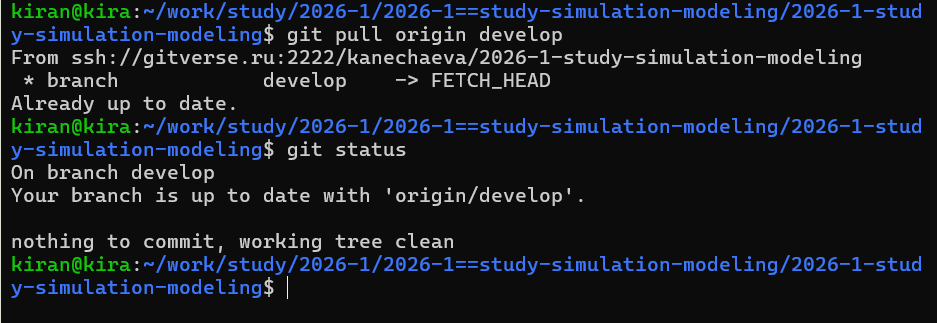
\includegraphics[width=0.9\linewidth,height=\textheight,keepaspectratio]{image/1.png}

}

\caption{Начало выполнения лабораторной работы № 4}

\end{figure}%

Для лабораторной работы использовалось отдельное окружение DrWatson.
Перед запуском экспериментов была проверена загрузка всех необходимых
библиотек.

\begin{figure}[H]

{\centering 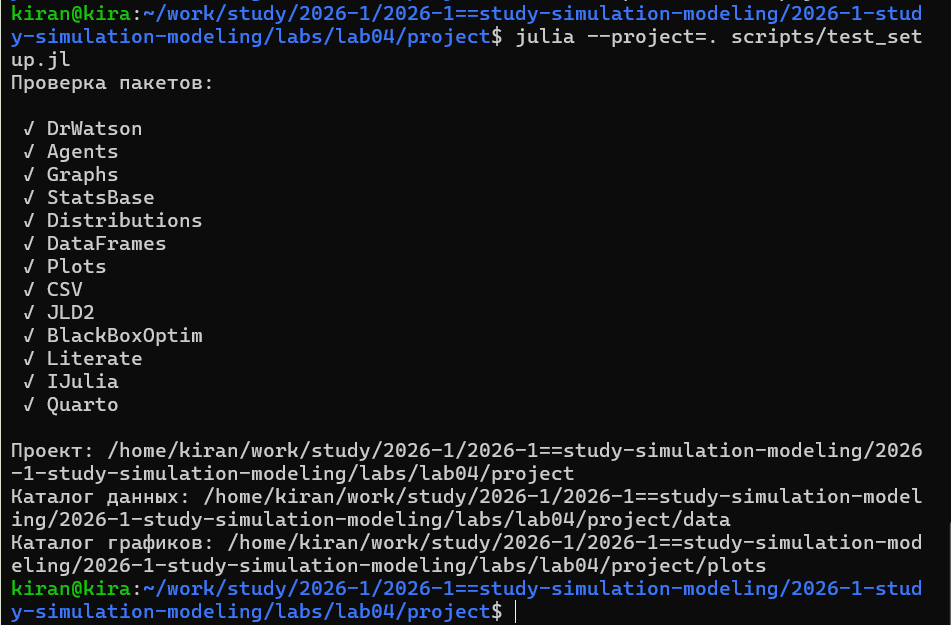
\includegraphics[width=0.9\linewidth,height=\textheight,keepaspectratio]{image/2.png}

}

\caption{Проверка программного окружения}

\end{figure}%

Основным инструментом агентного моделирования является пакет
\texttt{Agents.jl}. Для представления системы городов используется
графовое пространство, а случайное количество новых заражений
моделируется с помощью распределения Пуассона.

\chapter{Проверка агентной
модели}\label{ux43fux440ux43eux432ux435ux440ux43aux430-ux430ux433ux435ux43dux442ux43dux43eux439-ux43cux43eux434ux435ux43bux438}

Перед проведением основных экспериментов модель была проверена на
уменьшенной популяции.

\begin{figure}[H]

{\centering 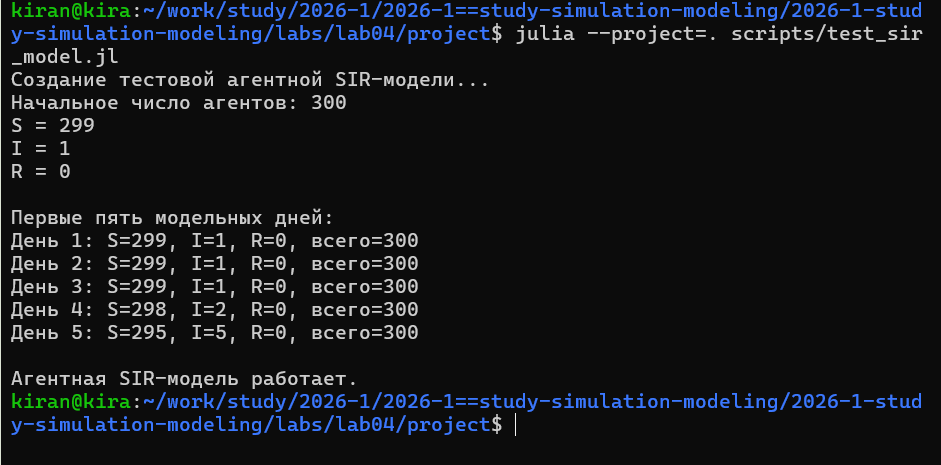
\includegraphics[width=0.9\linewidth,height=\textheight,keepaspectratio]{image/3.png}

}

\caption{Проверка ядра агентной модели SIR}

\end{figure}%

На тестовом запуске проверяется создание агентов, их распределение по
состояниям S, I и R и выполнение последовательных модельных шагов.

\chapter{Базовый
эксперимент}\label{ux431ux430ux437ux43eux432ux44bux439-ux44dux43aux441ux43fux435ux440ux438ux43cux435ux43dux442}

Базовая модель включает три города по 1000 агентов. Начальная инфекция
присутствует только у одного агента.

Для эксперимента программно вычисляется величина

\[
\gamma = \frac{1}{T},
\]

где \(T\) --- продолжительность инфекционного периода, а затем
определяется базовое репродуктивное число.

Также автоматически определяются эпидемический пик, день его достижения
и количество выбывших из-за смерти агентов.

\begin{figure}[H]

{\centering 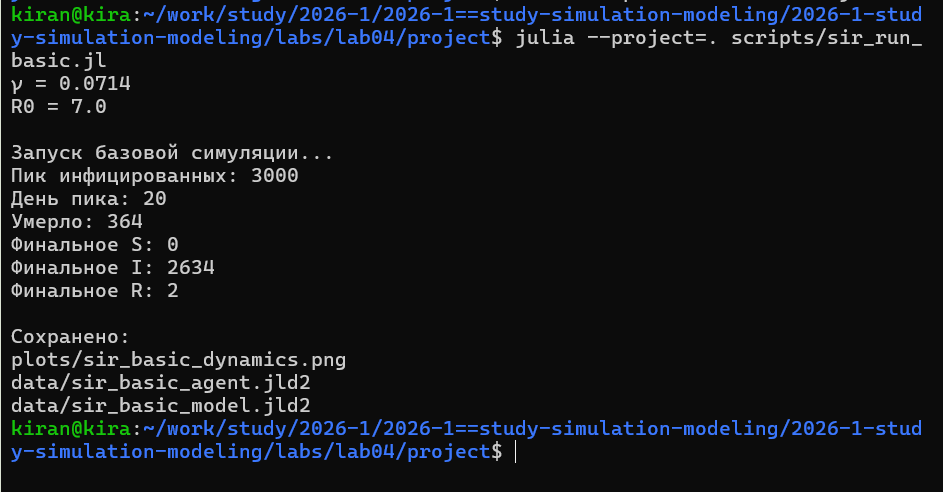
\includegraphics[width=0.9\linewidth,height=\textheight,keepaspectratio]{image/4.png}

}

\caption{Результаты базового запуска агентной SIR-модели}

\end{figure}%

Полученная динамика представлена на графике.

\begin{figure}[H]

{\centering 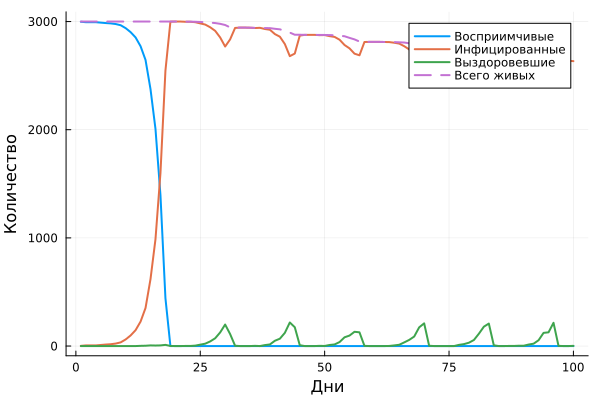
\includegraphics[width=0.85\linewidth,height=\textheight,keepaspectratio]{image/plots/sir_basic_dynamics.png}

}

\caption{Динамика состояний S, I и R}

\end{figure}%

В начале эксперимента большинство населения относится к состоянию S.
После появления инфекции количество I увеличивается, достигает максимума
и затем сокращается по мере перехода агентов в состояние R.

\section{Литературная версия базового
эксперимента}\label{ux43bux438ux442ux435ux440ux430ux442ux443ux440ux43dux430ux44f-ux432ux435ux440ux441ux438ux44f-ux431ux430ux437ux43eux432ux43eux433ux43e-ux44dux43aux441ux43fux435ux440ux438ux43cux435ux43dux442ux430}

Документация Quarto сформирована автоматически и сохранена в файле
\texttt{../project/markdown/sir\_run\_basic/sir\_run\_basic.qmd}.

\chapter{Исследование коэффициента
заразности}\label{ux438ux441ux441ux43bux435ux434ux43eux432ux430ux43dux438ux435-ux43aux43eux44dux444ux444ux438ux446ux438ux435ux43dux442ux430-ux437ux430ux440ux430ux437ux43dux43eux441ux442ux438}

Для анализа чувствительности модели коэффициент заразности изменялся от
0.1 до 1.0.

Поскольку агентная модель является стохастической, для каждого значения
выполнялось три прогона с различными значениями \texttt{seed}.

После этого показатели усреднялись.

\begin{figure}[H]

{\centering 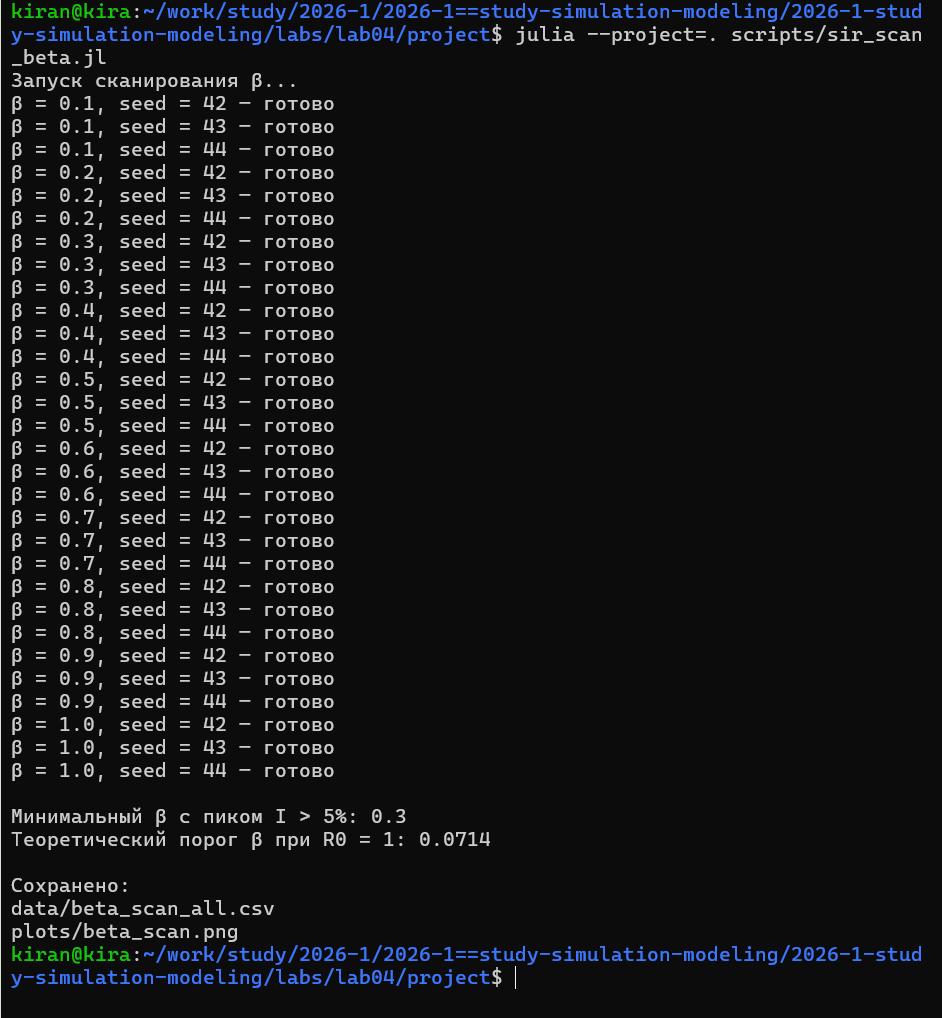
\includegraphics[width=0.9\linewidth,height=\textheight,keepaspectratio]{image/5.png}

}

\caption{Выполнение параметрического сканирования коэффициента
заразности}

\end{figure}%

Программа автоматически определяет минимальное значение коэффициента,
при котором пиковая доля инфицированных превышает 5 процентов, и
сравнивает его с теоретическим порогом.

\begin{figure}[H]

{\centering 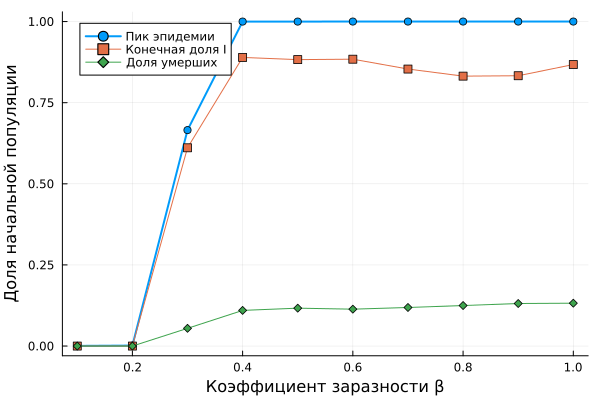
\includegraphics[width=0.85\linewidth,height=\textheight,keepaspectratio]{image/plots/beta_scan.png}

}

\caption{Влияние коэффициента заразности на развитие эпидемии}

\end{figure}%

Рост коэффициента заразности увеличивает эпидемическую нагрузку и влияет
на долю умерших.

\section{Литературная версия
исследования}\label{ux43bux438ux442ux435ux440ux430ux442ux443ux440ux43dux430ux44f-ux432ux435ux440ux441ux438ux44f-ux438ux441ux441ux43bux435ux434ux43eux432ux430ux43dux438ux44f}

Документация Quarto сформирована автоматически и сохранена в файле
\texttt{../project/markdown/sir\_scan\_beta/sir\_scan\_beta.qmd}.

\chapter{Гетерогенность
городов}\label{ux433ux435ux442ux435ux440ux43eux433ux435ux43dux43dux43eux441ux442ux44c-ux433ux43eux440ux43eux434ux43eux432}

В следующем эксперименте предположение об одинаковой заразности во всех
городах было снято.

Для трёх городов использовались различные значения коэффициента:

\begin{itemize}
\tightlist
\item
  первый город --- 0.2;
\item
  второй город --- 0.5;
\item
  третий город --- 0.8.
\end{itemize}

\begin{figure}[H]

{\centering 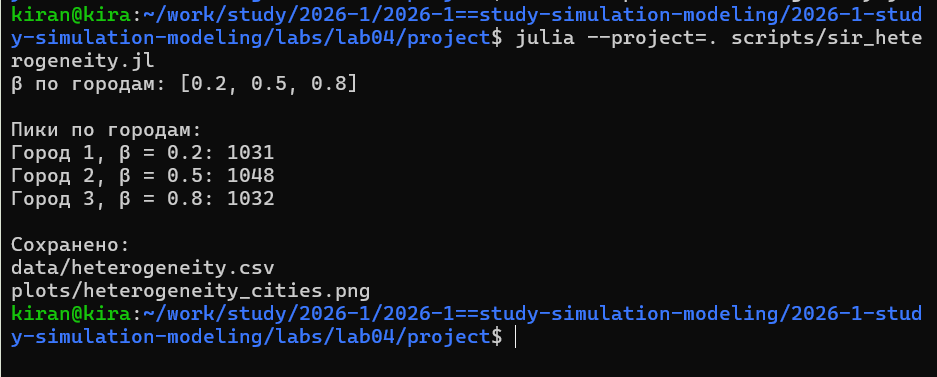
\includegraphics[width=0.9\linewidth,height=\textheight,keepaspectratio]{image/6.png}

}

\caption{Результаты эксперимента с различными коэффициентами заразности}

\end{figure}%

Динамика каждого города собиралась отдельно.

\begin{figure}[H]

{\centering 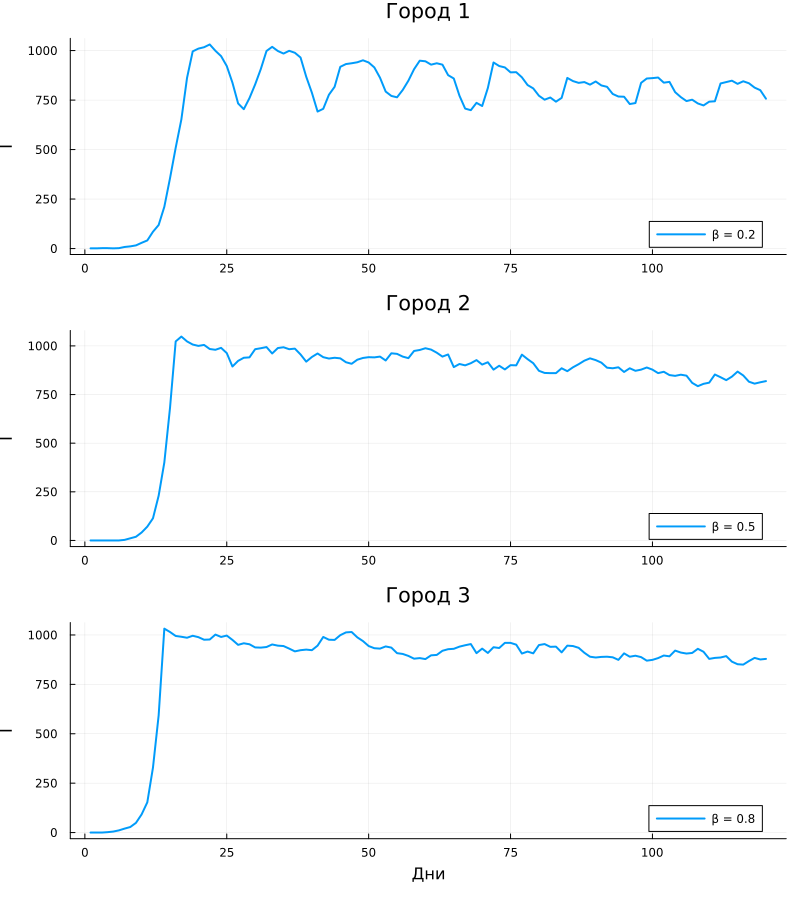
\includegraphics[width=0.82\linewidth,height=\textheight,keepaspectratio]{image/plots/heterogeneity_cities.png}

}

\caption{Динамика инфицированных в городах с различными коэффициентами
заразности}

\end{figure}%

Такой эксперимент показывает, что локальные характеристики отдельных
частей системы могут существенно изменять общую эпидемическую динамику.

\section{Литературная версия
эксперимента}\label{ux43bux438ux442ux435ux440ux430ux442ux443ux440ux43dux430ux44f-ux432ux435ux440ux441ux438ux44f-ux44dux43aux441ux43fux435ux440ux438ux43cux435ux43dux442ux430}

Документация Quarto сформирована автоматически и сохранена в файле
\texttt{../project/markdown/sir\_heterogeneity/sir\_heterogeneity.qmd}.

\chapter{Влияние
миграции}\label{ux432ux43bux438ux44fux43dux438ux435-ux43cux438ux433ux440ux430ux446ux438ux438}

В агентной модели агенты могут перемещаться между городами.

Для анализа этого эффекта интенсивность миграции изменялась от 0 до 0.5.

Для каждого значения выполнялось несколько независимых прогонов, после
чего рассчитывались среднее время до эпидемического пика и средняя
величина пика.

\begin{figure}[H]

{\centering 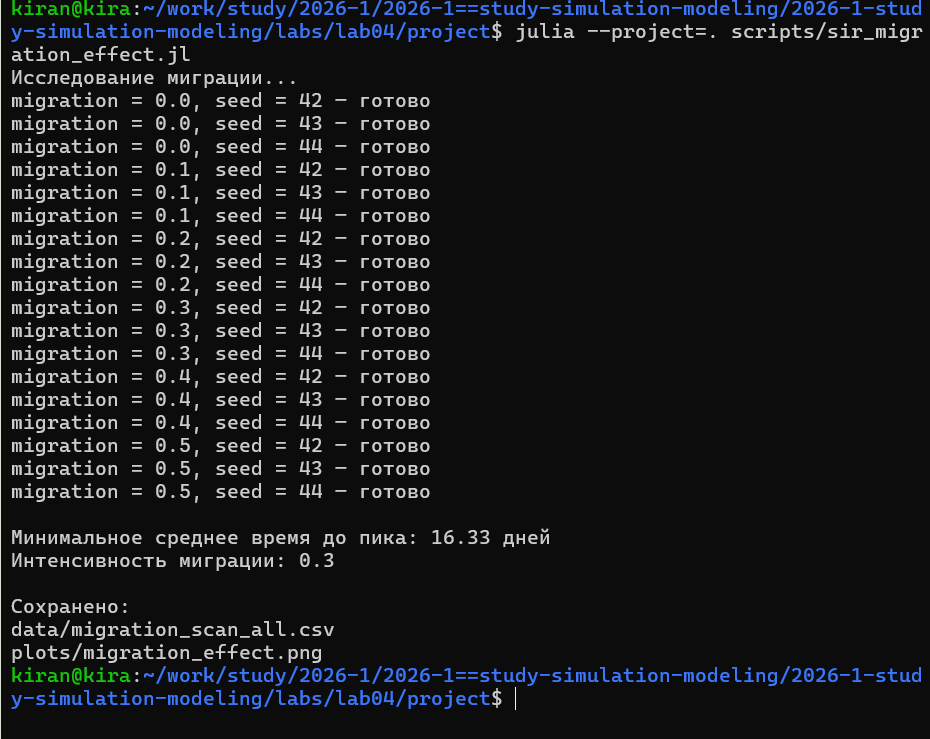
\includegraphics[width=0.9\linewidth,height=\textheight,keepaspectratio]{image/7.png}

}

\caption{Выполнение исследования интенсивности миграции}

\end{figure}%

Полученные зависимости:

\begin{figure}[H]

{\centering 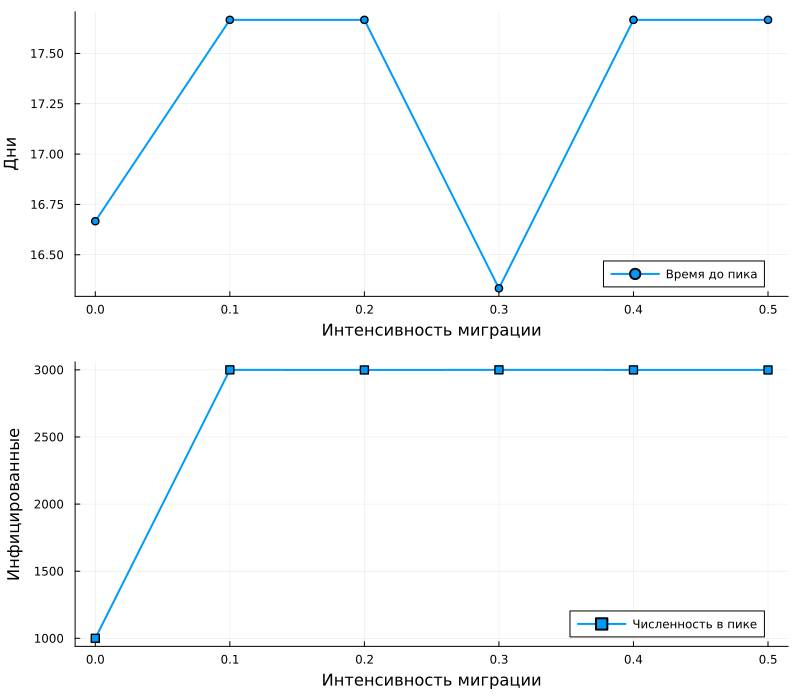
\includegraphics[width=0.85\linewidth,height=\textheight,keepaspectratio]{image/plots/migration_effect.png}

}

\caption{Влияние миграции на время и величину эпидемического пика}

\end{figure}%

Изменение мобильности населения влияет не только на масштаб эпидемии, но
и на скорость её распространения.

\section{Литературная версия
эксперимента}\label{ux43bux438ux442ux435ux440ux430ux442ux443ux440ux43dux430ux44f-ux432ux435ux440ux441ux438ux44f-ux44dux43aux441ux43fux435ux440ux438ux43cux435ux43dux442ux430-1}

Документация Quarto сформирована автоматически и сохранена в файле
\texttt{../project/markdown/sir\_migration\_effect/sir\_migration\_effect.qmd}.

\chapter{Карантинная
мера}\label{ux43aux430ux440ux430ux43dux442ux438ux43dux43dux430ux44f-ux43cux435ux440ux430}

В модель была добавлена возможность автоматически закрывать город при
превышении заданного порога заболеваемости.

При достижении долей инфицированных 10 процентов миграция из
соответствующего города блокируется.

Для корректного сравнения сценарии с карантином и без карантина
запускаются с одинаковым \texttt{seed}.

\begin{figure}[H]

{\centering 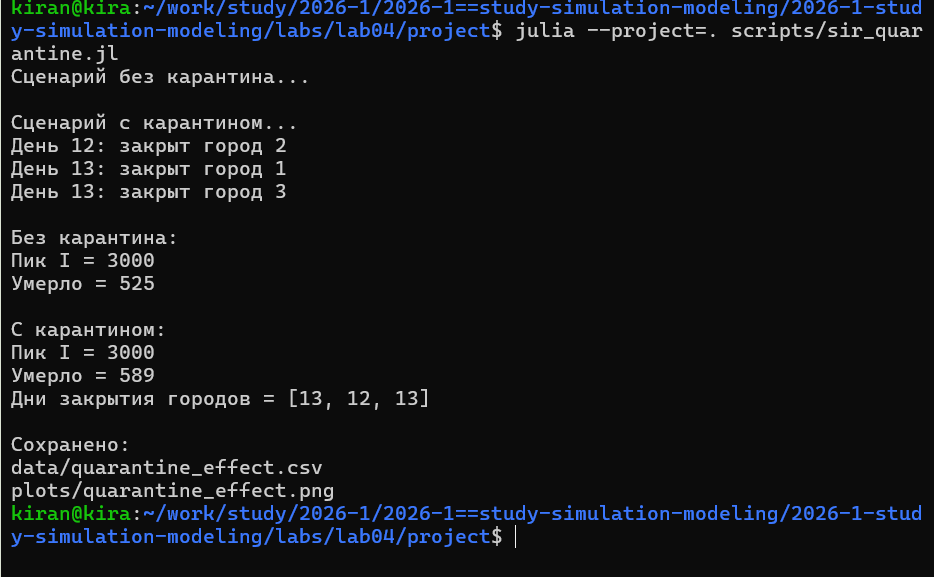
\includegraphics[width=0.9\linewidth,height=\textheight,keepaspectratio]{image/8.png}

}

\caption{Результаты эксперимента с карантинной мерой}

\end{figure}%

На графике сравниваются два сценария.

\begin{figure}[H]

{\centering 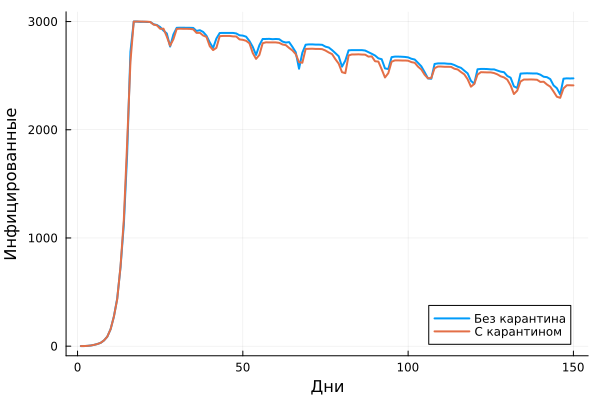
\includegraphics[width=0.85\linewidth,height=\textheight,keepaspectratio]{image/plots/quarantine_effect.png}

}

\caption{Сравнение эпидемической динамики с карантином и без него}

\end{figure}%

Такое сравнение позволяет оценить влияние ограничения мобильности на
эпидемический пик.

\section{Литературная версия
эксперимента}\label{ux43bux438ux442ux435ux440ux430ux442ux443ux440ux43dux430ux44f-ux432ux435ux440ux441ux438ux44f-ux44dux43aux441ux43fux435ux440ux438ux43cux435ux43dux442ux430-2}

Документация Quarto сформирована автоматически и сохранена в файле
\texttt{../project/markdown/sir\_quarantine/sir\_quarantine.qmd}.

\chapter{Оптимизация
параметров}\label{ux43eux43fux442ux438ux43cux438ux437ux430ux446ux438ux44f-ux43fux430ux440ux430ux43cux435ux442ux440ux43eux432}

Для поиска допустимой стратегии управления была выполнена автоматическая
оптимизация параметров модели.

Оптимизатор изменяет:

\begin{itemize}
\tightlist
\item
  коэффициент заразности;
\item
  время выявления заболевания;
\item
  параметр смертности.
\end{itemize}

Целевая функция минимизирует смертность, при этом превышение пикового
уровня инфицированных в 30 процентов штрафуется.

\begin{figure}[H]

{\centering 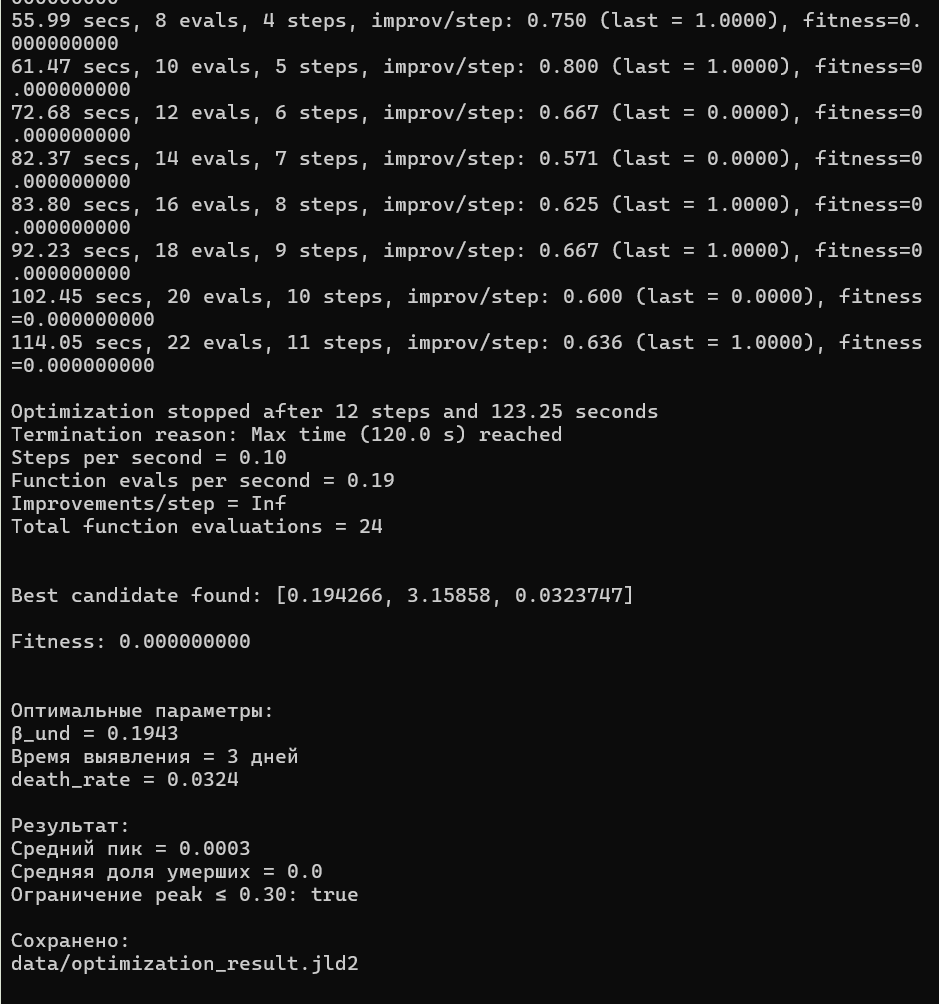
\includegraphics[width=0.9\linewidth,height=\textheight,keepaspectratio]{image/9.png}

}

\caption{Результат оптимизации параметров агентной SIR-модели}

\end{figure}%

После завершения оптимизации программа повторно оценивает найденный
набор параметров на нескольких независимых прогонах.

\section{Литературная версия
оптимизации}\label{ux43bux438ux442ux435ux440ux430ux442ux443ux440ux43dux430ux44f-ux432ux435ux440ux441ux438ux44f-ux43eux43fux442ux438ux43cux438ux437ux430ux446ux438ux438}

Документация Quarto сформирована автоматически и сохранена в файле
\texttt{../project/markdown/sir\_optimize\_parameters/sir\_optimize\_parameters.qmd}.

\chapter{Сводная
визуализация}\label{ux441ux432ux43eux434ux43dux430ux44f-ux432ux438ux437ux443ux430ux43bux438ux437ux430ux446ux438ux44f}

Для итогового анализа использовались ранее сохранённые результаты
сканирования коэффициента заразности.

Повторный запуск всех симуляций для этого этапа не требуется.

\begin{figure}[H]

{\centering 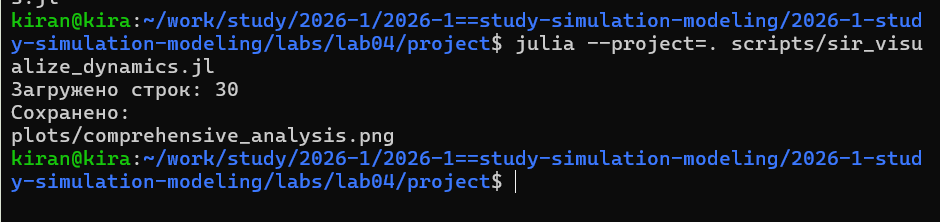
\includegraphics[width=0.9\linewidth,height=\textheight,keepaspectratio]{image/10.png}

}

\caption{Создание сводной визуализации}

\end{figure}%

Итоговая фигура объединяет информацию о пике инфекции, смертности и доле
выздоровевших.

\begin{figure}[H]

{\centering 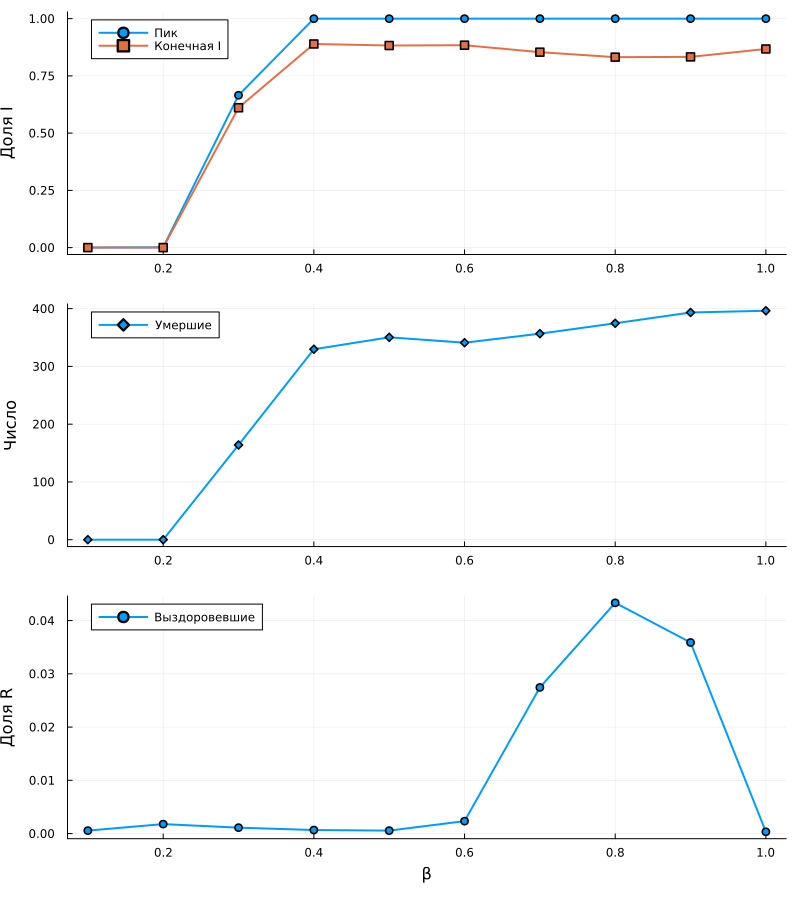
\includegraphics[width=0.82\linewidth,height=\textheight,keepaspectratio]{image/plots/comprehensive_analysis.png}

}

\caption{Сводный анализ результатов параметрического исследования}

\end{figure}%

\section{Литературная версия
визуализации}\label{ux43bux438ux442ux435ux440ux430ux442ux443ux440ux43dux430ux44f-ux432ux435ux440ux441ux438ux44f-ux432ux438ux437ux443ux430ux43bux438ux437ux430ux446ux438ux438}

Документация Quarto сформирована автоматически и сохранена в файле
\texttt{../project/markdown/sir\_visualize\_dynamics/sir\_visualize\_dynamics.qmd}.

\chapter{Генерация производных
форматов}\label{ux433ux435ux43dux435ux440ux430ux446ux438ux44f-ux43fux440ux43eux438ux437ux432ux43eux434ux43dux44bux445-ux444ux43eux440ux43cux430ux442ux43eux432}

Все основные программы были оформлены в литературном стиле.

Для каждой из них автоматически сформированы:

\begin{itemize}
\tightlist
\item
  чистый Julia-код;
\item
  документ Quarto;
\item
  Jupyter Notebook.
\end{itemize}

\begin{figure}[H]

{\centering 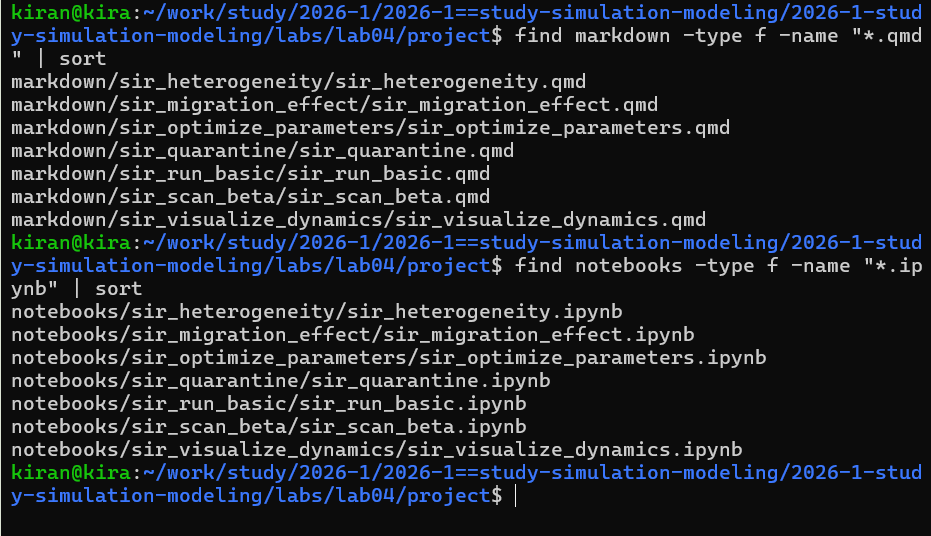
\includegraphics[width=0.9\linewidth,height=\textheight,keepaspectratio]{image/11.png}

}

\caption{Автоматически сформированные Quarto-документы и notebooks}

\end{figure}%

\chapter{Проверка
воспроизводимости}\label{ux43fux440ux43eux432ux435ux440ux43aux430-ux432ux43eux441ux43fux440ux43eux438ux437ux432ux43eux434ux438ux43cux43eux441ux442ux438}

Сгенерированные Jupyter Notebook были повторно выполнены.

\begin{figure}[H]

{\centering 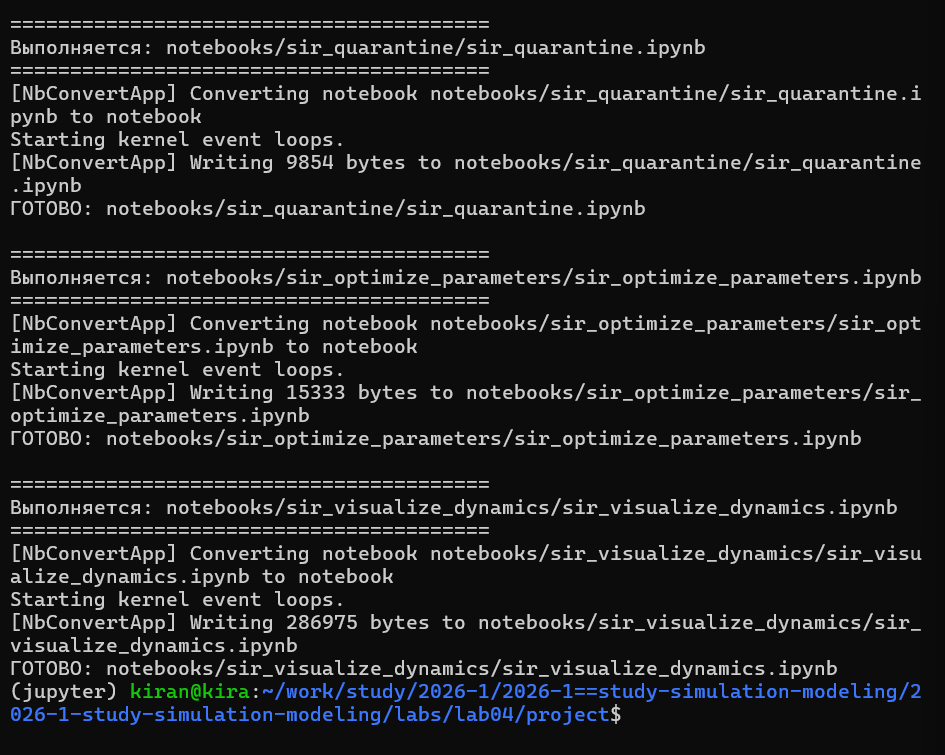
\includegraphics[width=0.9\linewidth,height=\textheight,keepaspectratio]{image/12.png}

}

\caption{Успешное выполнение Jupyter Notebook}

\end{figure}%

Таким образом была проверена воспроизводимость вычислительных
экспериментов из автоматически созданных notebooks.

\chapter{Итоговая структура
проекта}\label{ux438ux442ux43eux433ux43eux432ux430ux44f-ux441ux442ux440ux443ux43aux442ux443ux440ux430-ux43fux440ux43eux435ux43aux442ux430}

После выполнения лабораторной работы в проекте сохранены:

\begin{itemize}
\tightlist
\item
  ядро агентной модели;
\item
  литературные исходники;
\item
  чистые Julia-скрипты;
\item
  Quarto-документация;
\item
  Jupyter Notebook;
\item
  CSV и JLD2-файлы с результатами;
\item
  оригинальные PNG-графики.
\end{itemize}

\begin{figure}[H]

{\centering 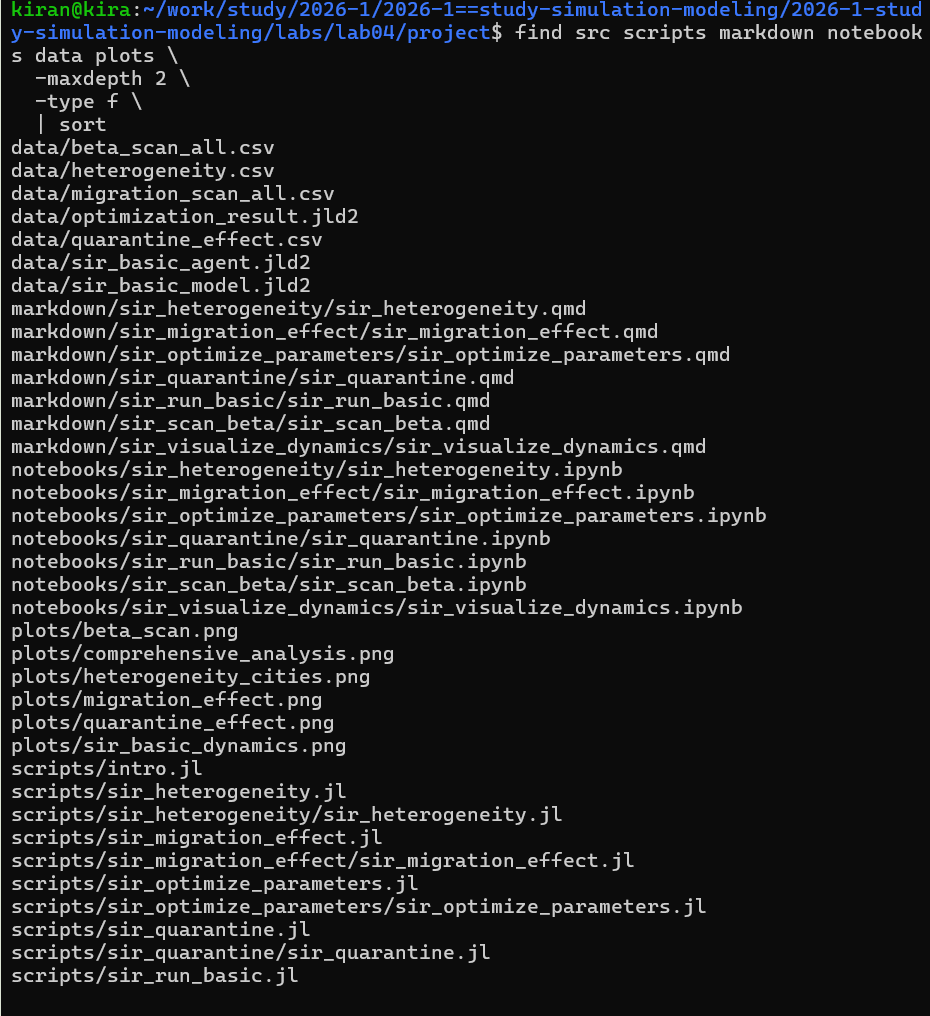
\includegraphics[width=0.9\linewidth,height=\textheight,keepaspectratio]{image/13.png}

}

\caption{Итоговая структура файлов лабораторной работы}

\end{figure}%

Все результаты были зафиксированы в системе контроля версий.

\begin{figure}[H]

{\centering 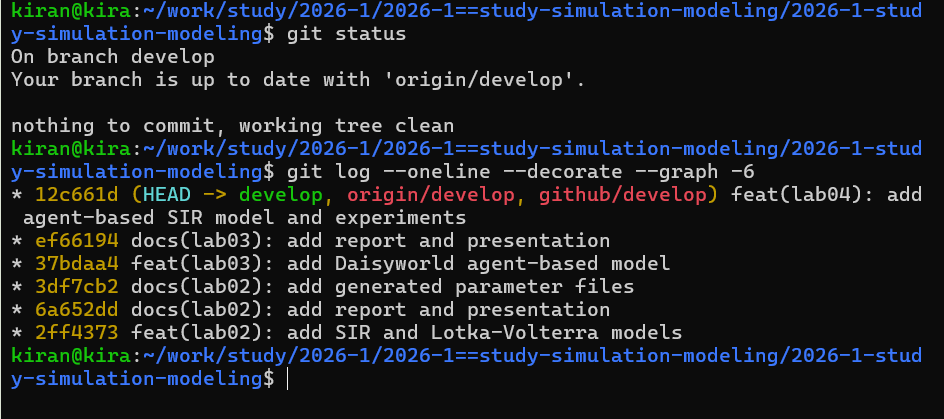
\includegraphics[width=0.9\linewidth,height=\textheight,keepaspectratio]{image/14.png}

}

\caption{Сохранение лабораторной работы в Git}

\end{figure}%

\chapter{Заключение}\label{ux437ux430ux43aux43bux44eux447ux435ux43dux438ux435}

В лабораторной работе классическая модель SIR была реализована в
агентном подходе.

Каждый индивид моделировался отдельно, а пространство было представлено
системой взаимосвязанных городов.

Были исследованы базовая динамика эпидемии, влияние коэффициента
заразности, гетерогенность городов и интенсивность миграции.

Дополнительно в модель была добавлена карантинная мера и выполнена
автоматическая оптимизация параметров.

Все основные вычисления выполнялись программно, а исходники были
оформлены в литературном стиле с автоматическим формированием Julia,
Quarto и Jupyter Notebook.


\printbibliography



\end{document}
